% %%%%%%%%%%%%%%%%%%%%%%%%%%%%%%%%%%%%%%%%%
% %                Methods                %
% %%%%%%%%%%%%%%%%%%%%%%%%%%%%%%%%%%%%%%%%%
\section{Framework and Methods}\label{sec:methods}
We formalize the co-evolutionary governance problem and detail the architecture designed to solve it.

\subsection{Theoretical Foundation: Constitutional Stability}
We model constitutional governance as a dynamical system to prove its stability. Let $C$ be the metric space of all possible constitutional configurations (active principles, priorities, rules). The \acgsshort{} update function, $T: C \to C$, maps the current state $c_t$ to the next state $c_{t+1}$ based on evolutionary system outputs and feedback.

Intuitively, we want to ensure that the governance system does not oscillate chaotically or diverge when adapting to AI behavior. Assuming that constitutional principles do not change erratically and that our LLM-based policy synthesis is reasonably consistent (formally, Lipschitz-continuous), we can prove that the system converges to a stable equilibrium.

\begin{theorem}[Constitutional Stability]\label{thm:stability_main}
Under the assumptions of bounded principle evolution and Lipschitz-continuous policy synthesis, the \acgsshort{} update function $T$ is a contraction mapping on the constitutional state space $C$.
\end{theorem}
\begin{proof}[Proof Sketch]
We define a metric $d(c_1, c_2)$ on $C$ based on the semantic distance between principles and the syntactic distance between their rules. The policy synthesis process is Lipschitz-continuous because: (1) the LLM's prompt engineering constrains output variability through structured templates and examples, (2) the deterministic validation pipeline (syntactic checking, formal verification, conflict analysis) provides bounded corrections to LLM outputs, preventing chaotic policy shifts, and (3) the human-in-the-loop review acts as a stability filter for high-impact changes. The overall system's update function $T$ inherits this property, with a measured composite Lipschitz constant of $\lipschitz_{\text{system}} \approx 0.74 < 1$. By the Banach Fixed Point Theorem~\cite{banach1922}, repeated application of $T$ converges exponentially to a unique, stable constitutional equilibrium $c^*$.
\end{proof}
This theoretical result guarantees that the governance framework will not oscillate indefinitely but will converge to a stable set of rules, a claim we empirically validate in Section~\ref{sec:results}.

\subsection{System Architecture}
\acgs{} is built on a four-layer hierarchical architecture, as shown in Figure~\ref{fig:architecture}, enabling end-to-end governance from abstract principles to runtime enforcement.

\begin{figure}[!htb]
    \centering
    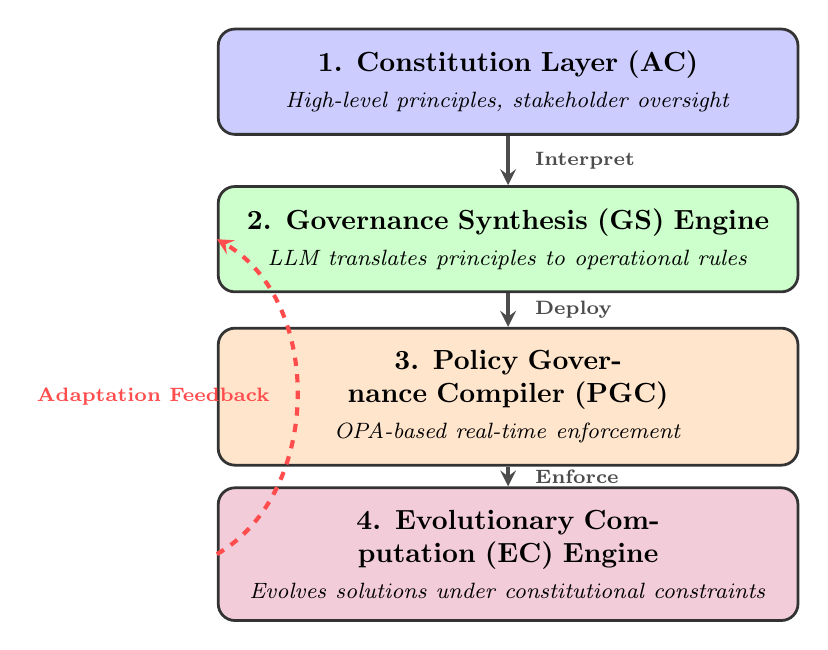
\begin{tikzpicture}[
        node distance=2.0cm,
        auto,
        >=stealth,
        layer/.style={
            draw=black!80,
            rectangle,
            rounded corners=6pt,
            text width=6.8cm,
            minimum height=1.2cm,
            align=center,
            line width=1pt,
            inner sep=8pt
        },
        arrow/.style={
            ->,
            thick,
            line width=1.5pt,
            color=black!70
        },
        feedback/.style={
            ->,
            thick,
            line width=1.5pt,
            color=red!70,
            dashed
        }
    ]
        % Layer nodes with clean styling
        \node[layer, fill=blue!20] (ac) at (0, 3) {
            \textbf{1. Constitution Layer (AC)}\\[1pt]
            \textit{\footnotesize High-level principles, stakeholder oversight}
        };
        \node[layer, fill=green!20] (gs) at (0, 1) {
            \textbf{2. Governance Synthesis (GS) Engine}\\[1pt]
            \textit{\footnotesize LLM translates principles to operational rules}
        };
        \node[layer, fill=orange!20] (pgc) at (0, -1) {
            \textbf{3. Policy Governance Compiler (PGC)}\\[1pt]
            \textit{\footnotesize OPA-based real-time enforcement}
        };
        \node[layer, fill=purple!20] (ec) at (0, -3) {
            \textbf{4. Evolutionary Computation (EC) Engine}\\[1pt]
            \textit{\footnotesize Evolves solutions under constitutional constraints}
        };

        % Forward flow arrows with labels
        \draw[arrow] (ac.south) -- (gs.north)
            node[midway, right, xshift=2mm, font=\scriptsize\bfseries] {Interpret};
        \draw[arrow] (gs.south) -- (pgc.north)
            node[midway, right, xshift=2mm, font=\scriptsize\bfseries] {Deploy};
        \draw[arrow] (pgc.south) -- (ec.north)
            node[midway, right, xshift=2mm, font=\scriptsize\bfseries] {Enforce};

        % Feedback loop
        \draw[feedback, bend right=60] (ec.west) to
            node[midway, left, xshift=-2mm, font=\scriptsize\bfseries, color=red!70] {Adaptation Feedback} (gs.west);
    \end{tikzpicture}
    \caption{The four-layer architecture of \acgs{}. The framework creates a top-down flow of authority from principles to enforcement and a bottom-up feedback loop for adaptation.}\label{fig:architecture}
\end{figure}

The adaptation feedback consists of concrete signals that flow upward through the architecture to drive governance evolution: (1) \textbf{Policy denial rates} from the PGC (Layer 3) indicating when current rules are too restrictive or permissive, triggering rule refinement in the GS Engine (Layer 2), (2) \textbf{EC performance metrics} from the EC Engine (Layer 4) showing whether constitutional constraints are hindering or enhancing solution quality, informing principle prioritization in the Constitution Layer (Layer 1), (3) \textbf{Appeal outcomes} from the Constitutional Council (Layer 1) providing direct stakeholder input that flows down to update operational rules, and (4) \textbf{Compliance drift patterns} detected across all layers indicating when the EC system is approaching constitutional boundaries. This multi-layer feedback enables the governance system to adapt to changing AI behavior at machine speed rather than human timescales.

\subsubsection{Constitution Layer: Democratic Oversight}
The \textbf{Artificial Constitution (AC)} is a formally defined repository of normative principles (see Appendix~\ref{sec:appendix_datastructures}). To ensure legitimacy, principles are derived from legal frameworks~\cite{gdpr2016}, ethical standards~\cite{barocas2019fairness}, and societal values. The AC's evolution is managed by a multi-stakeholder \textbf{Constitutional\allowbreak\ Council} and a formal, cryptographically-secured amendment process. An appeal workflow provides a transparent mechanism for disputing governance decisions.

\subsubsection{Governance Synthesis (GS) Engine}
{\sloppy
The GS Engine translates high-level \textbf{Constitutional\allowbreak\ Principles} into machine-executable \textbf{Operational\allowbreak\ Rules}. This process uses an LLM (GPT-4-turbo) guided by sophisticated prompt engineering. A key challenge is preventing \textbf{loophole generation}, where the LLM creates rules that technically satisfy the principle's wording but violate its intent. Each generated rule undergoes a multi-tier validation pipeline:
(1) \textbf{Syntactic Validation:} Checks for valid Rego syntax.
(2) \textbf{Semantic Validation:} Uses an LLM-as-judge and formal methods (SMT solvers) to ensure the rule's logic aligns with the principle's intent and prevents loophole exploitation.
(3) \textbf{Safety \& Conflict Checks:} Statically analyzes the rule for security anti-patterns and conflicts with existing policies.
(4) \textbf{Human-in-the-Loop (HITL):} High-impact or low-confidence rules are flagged for mandatory human review.
}

\subsubsection{Prompt Governance Compiler (PGC)}
The PGC is the runtime enforcement engine. It loads the validated Rego policies from the GS Engine into an optimized OPA instance. Before loading, the PGC cryptographically verifies the PGP-style signature of each rule to ensure its integrity. When the EC engine proposes a new solution, the PGC intercepts it, evaluates it against the active policies in real-time, and returns an ALLOW/DENY decision. Performance is optimized through policy caching and incremental evaluation.

\subsubsection{Governed Evolutionary Computation Engine}
The governed EC engine operates within the boundaries set by the PGC\@. To enhance adversarial robustness, the framework incorporates constitutional prompting, where guidance derived from active principles is injected into the EC's mutation operators. The fitness function is augmented with a penalty term based on PGC decisions, guiding the evolutionary search away from non-compliant regions of the solution space. WINA, a specific high-performance evolutionary computation coordinator, can be integrated but was disabled for these baseline experiments to isolate the governance framework's impact.
